\documentclass{article}
\usepackage{longtable}
\usepackage{booktabs}
\usepackage{todonotes}
\usepackage{url}
\usepackage[hidelinks,breaklinks=true]{hyperref}
\usepackage{geometry}
\usepackage{graphicx}
\usepackage{float}
\graphicspath{ {./images/} }
\geometry{margin=1in}

% Define tightlist for pandoc compatibility
\providecommand{\tightlist}{%
  \setlength{\itemsep}{0pt}\setlength{\parskip}{0pt}}

\begin{document}

\section{PATh Supplement - Status and Progress of Hetergeneous Model
Training}\label{path-supplement---status-and-progress-of-hetergeneous-model-training}

\subsection{Objectives}\label{objectives}


As a supplement to the Partnership to Advanced Throughput Computing
(PATh) project, we have launched a new collaboration with a group of
domain scientists and ML researchers to run a pathfinder project
profiling the effects of throughput training and inference on
distributed, heterogeneous capacity. The goals of this activity, are
threefold:

\begin{enumerate}
\tightlist
\item{Characterize the impact of training ensembles across heterogeneous
resources, as opposed to the traditional approach of ``single
homogeneous cluster''.}
\item{Use the workloads developed in (1) to improve capabilities and
services, reducing the barrier of entry for new ML researchers to use
the PATh services to train ensembles with capacity powered by the NAIRR
pilot.}
\item{Demonstrate running single workloads managed by a single Access Point
(AP) effectively across as many of the NAIRR pilot resources as
possible.}
\end{enumerate}

To accomplish these goals, we will use the existing Gitter lab's
published Mutational Effect Transfer Learning (METL) protein language
model, using existing data and software to train a modest number of
model variants (20-30) from a single AP, intentionally moving the
training processes between available resources. Comparison of these
variants will prove compatibility of the models, ensuring that the
heterogeneity of resources did not impact the scientific power of the
models.

\subsection{Methodology}\label{methodology}

\subsubsection{NAIRR allocations}\label{nairr-allocations}

Through the NAIRR pilot program, we applied (NAIRR240335) for and
received allocations at 6 sites:

\begin{longtable}[]{@{}ll@{}}
\toprule\noalign{}
Site & Approved allocation \\
\midrule\noalign{}
\endhead
\endlastfoot
NCSA Delta GPU & 11,500 GPU hours \\
Amazon Web Services & \$6,300 \\
Indiana Jetstream2 GPU & 86,016 SUs \\
PSC Bridges-2 GPU & 1,500 GPU hours \\
Purdue Anvil GPU & 1,500 GPU hours \\
SDSC Expanse GPU & 1,500 GPU hours \\
\bottomrule\noalign{}
\end{longtable}

\subsubsection{Access Point}\label{access-point}

We used the OSPool access point
\href{http://ap40.uw.osg-htc.org}{\texttt{ap40.uw.osg-htc.org}} for this
initial round of experiments. In parallel, a machine dedicated for the
PATh supplement was ordered and is currently being configured as of
2025-07-30). There is no special configuration needed on this machine to
enable utilization of the NAIRR resources beyond the pre-existing
configuration to enable HTCondor Annex creation (described below).

\subsubsection{Job description}\label{job-description}

The METL software is well-documented and publicly available via github
(\url{https://github.com/gitter-lab/metl/}). Input data and conda
environments are similarly available within Zenodo
(\url{https://zenodo.org/records/14916528}).\\
In order to ease the distribution and deployment of the training
software, a Docker container image was created
(\url{https://github.com/CHTC/METL-Conductor/blob/main/Dockerfile})
which contains the installed software. This image was then converted
into an apptainer image. The apptainer and input data were then stored
within the OSDF to ease the movement across the computing ecosystem.
Total input sizes are \textasciitilde6GB for the image and
$\sim$20GB for the data.\\
Initial benchmarking of the training task was first tested locally on
V100 machines, giving approximate resource needs. Additional
benchmarking was done both in the CHTC and OSPool clusters to further
test and understand the performance and resource needs of the training
process.\\
Finally, test jobs were run within the targeted NAIRR sites to comb out
the differences between the sites and to dial in the resource
requirements within the job definitions needed for each.
An initial training model (uuid 861e7e66) was trained, alternating between
Expanse and Delta annexes.

\subsubsection{HTCondor Annex}\label{htcondor-annex}

In order to provide single-AP access to the NAIRR sites, we used
HTCondor's Annex feature. This tool submits a pilot job (or jobs) into a
remote site based on the resource requests (and desired number of nodes)
from the researcher. These jobs leverage the sites' local scheduling
software and, upon starting, will create an HTCondor Execution Point
(EP) that become available within the researcher's local cluster to run
their job lists.\\
Minor development was needed within the annex software, primarily to
update the partition definitions and settings at the remote sites. The
AWS annex required additional development to run an Amazon Machine Image
(AMI) compatible with GPU usage.

\subsubsection{DAG}\label{dag}

Building upon a previous summer fellow's work, we create a DAG generator
script, in order to:

\begin{enumerate}
\tightlist
\item
  Organize and automate the workload\\
\item
  Identify common patterns of scripted DAG generations\\
\item
  From 2, understand the shortcomings of DAGMan within the context of
  throughput training tasks (ensemble training, hyperparameter sweeps)
\end{enumerate}

The DAG itself is an array of ``shish-kebab'' subgraphs, with each node
defining a single job, itself defined as a single epoch of training.
Evaluation of validation data was done within the training job, though
the generation script supports separate side-nodes for evaluation.

\begin{figure}[H]
\centering
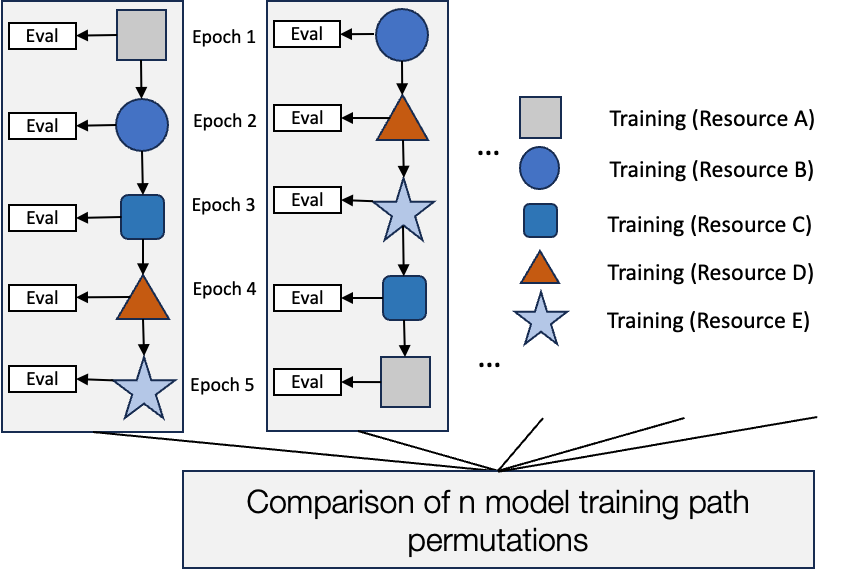
\includegraphics[width=0.8\textwidth]{DAG}
\label{fig:dag}
\caption{A diagram showing the shape of the DAG implemented. The diagram
shows 2 training runs, each of 5 epochs, for simplicity.}
\end{figure}

\todo{monitoring}

\subsection{Results}\label{results}
\subsubsection{Training process}\label{results_training}

In total,
5,318.6 GPU hours were utilized
Six different GPU models were utilized:

\begin{table}[h]
\centering
\begin{tabular}{|c|c|}
\hline
GPU Model & Epochs trained \\ \hline

A100-PCIE-40GB & 6  \\ \hline
A100-SXM4-40GB & 43 \\ \hline
A100-SXM4-80GB & 73 \\ \hline
A40 & 108 \\ \hline
RTX A5000 & 354 \\ \hline
V100-XSM2-32GB & 46 \\ \hline
\end{tabular}
\caption{GPU Utilization Breakdown}
\label{tab:gpu_utilization}
\end{table}

\begin{figure}[H]
\centering
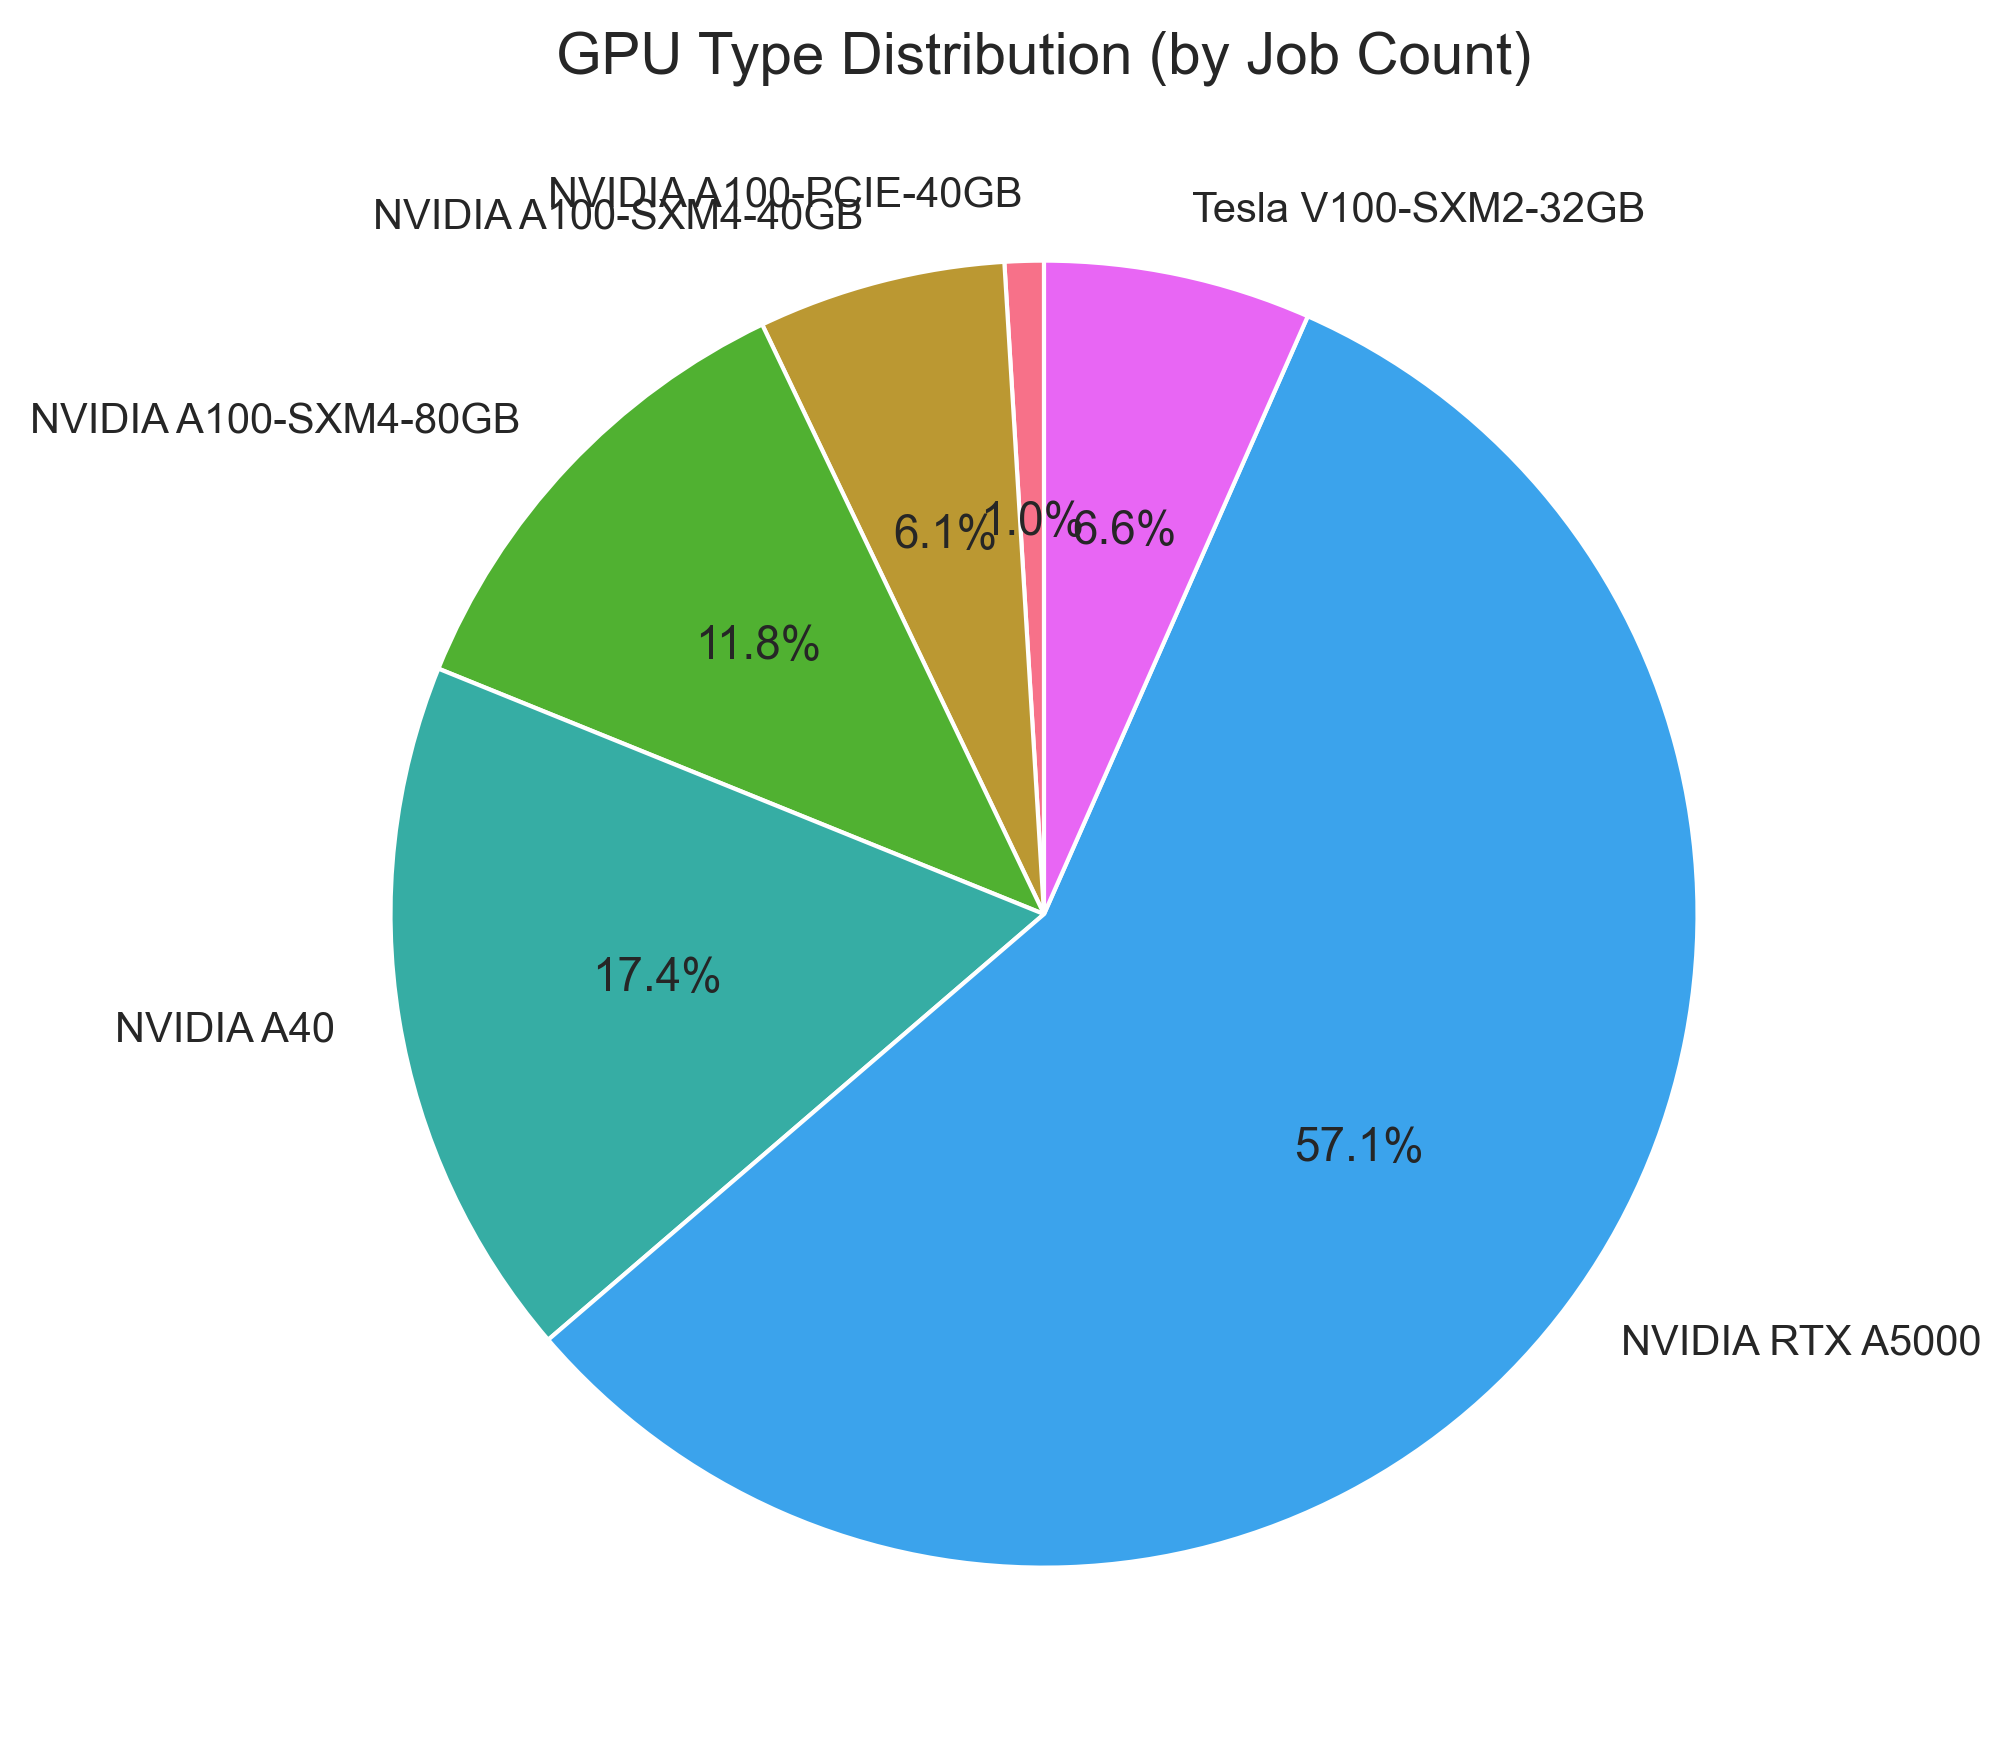
\includegraphics[width=0.8\textwidth]{gpu_distribution_analysis.png}
\label{fig:gpu_distribution}
\caption{Distribution of epochs by GPU model.}
\end{figure}

\begin{figure}[H]
\centering
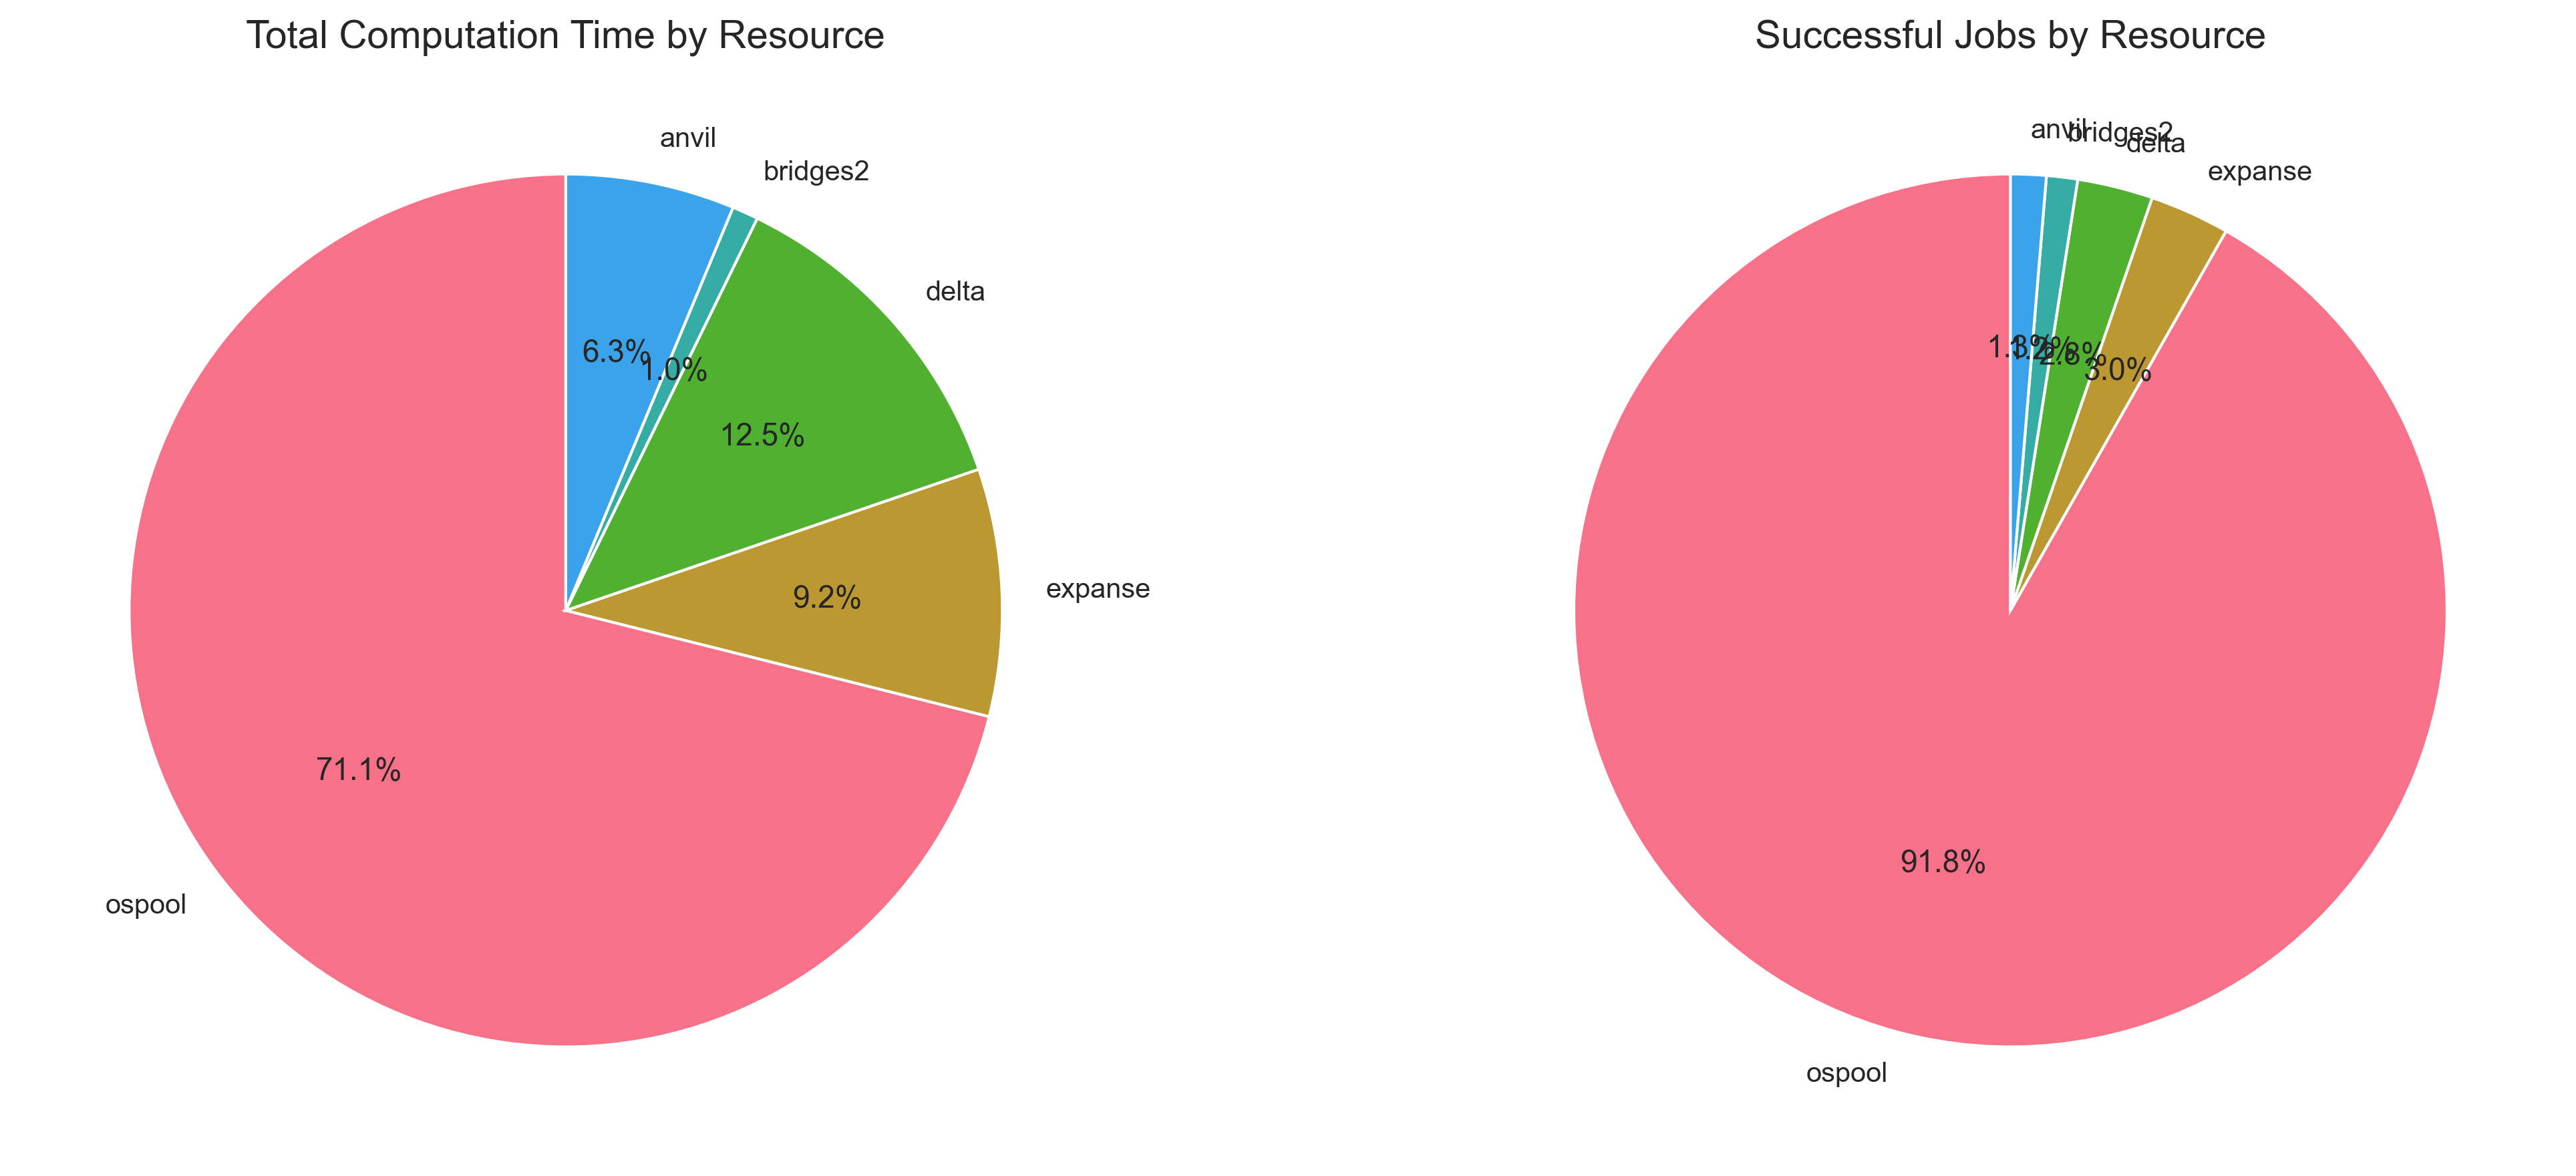
\includegraphics[width=0.8\textwidth]{resource_time_breakdown.png}
\label{fig:resource_time_breakdown}
\caption{Distribution of training time (left) and epochs trained (right) by targeted resource.}
\end{figure}

\begin{figure}[H]
\centering
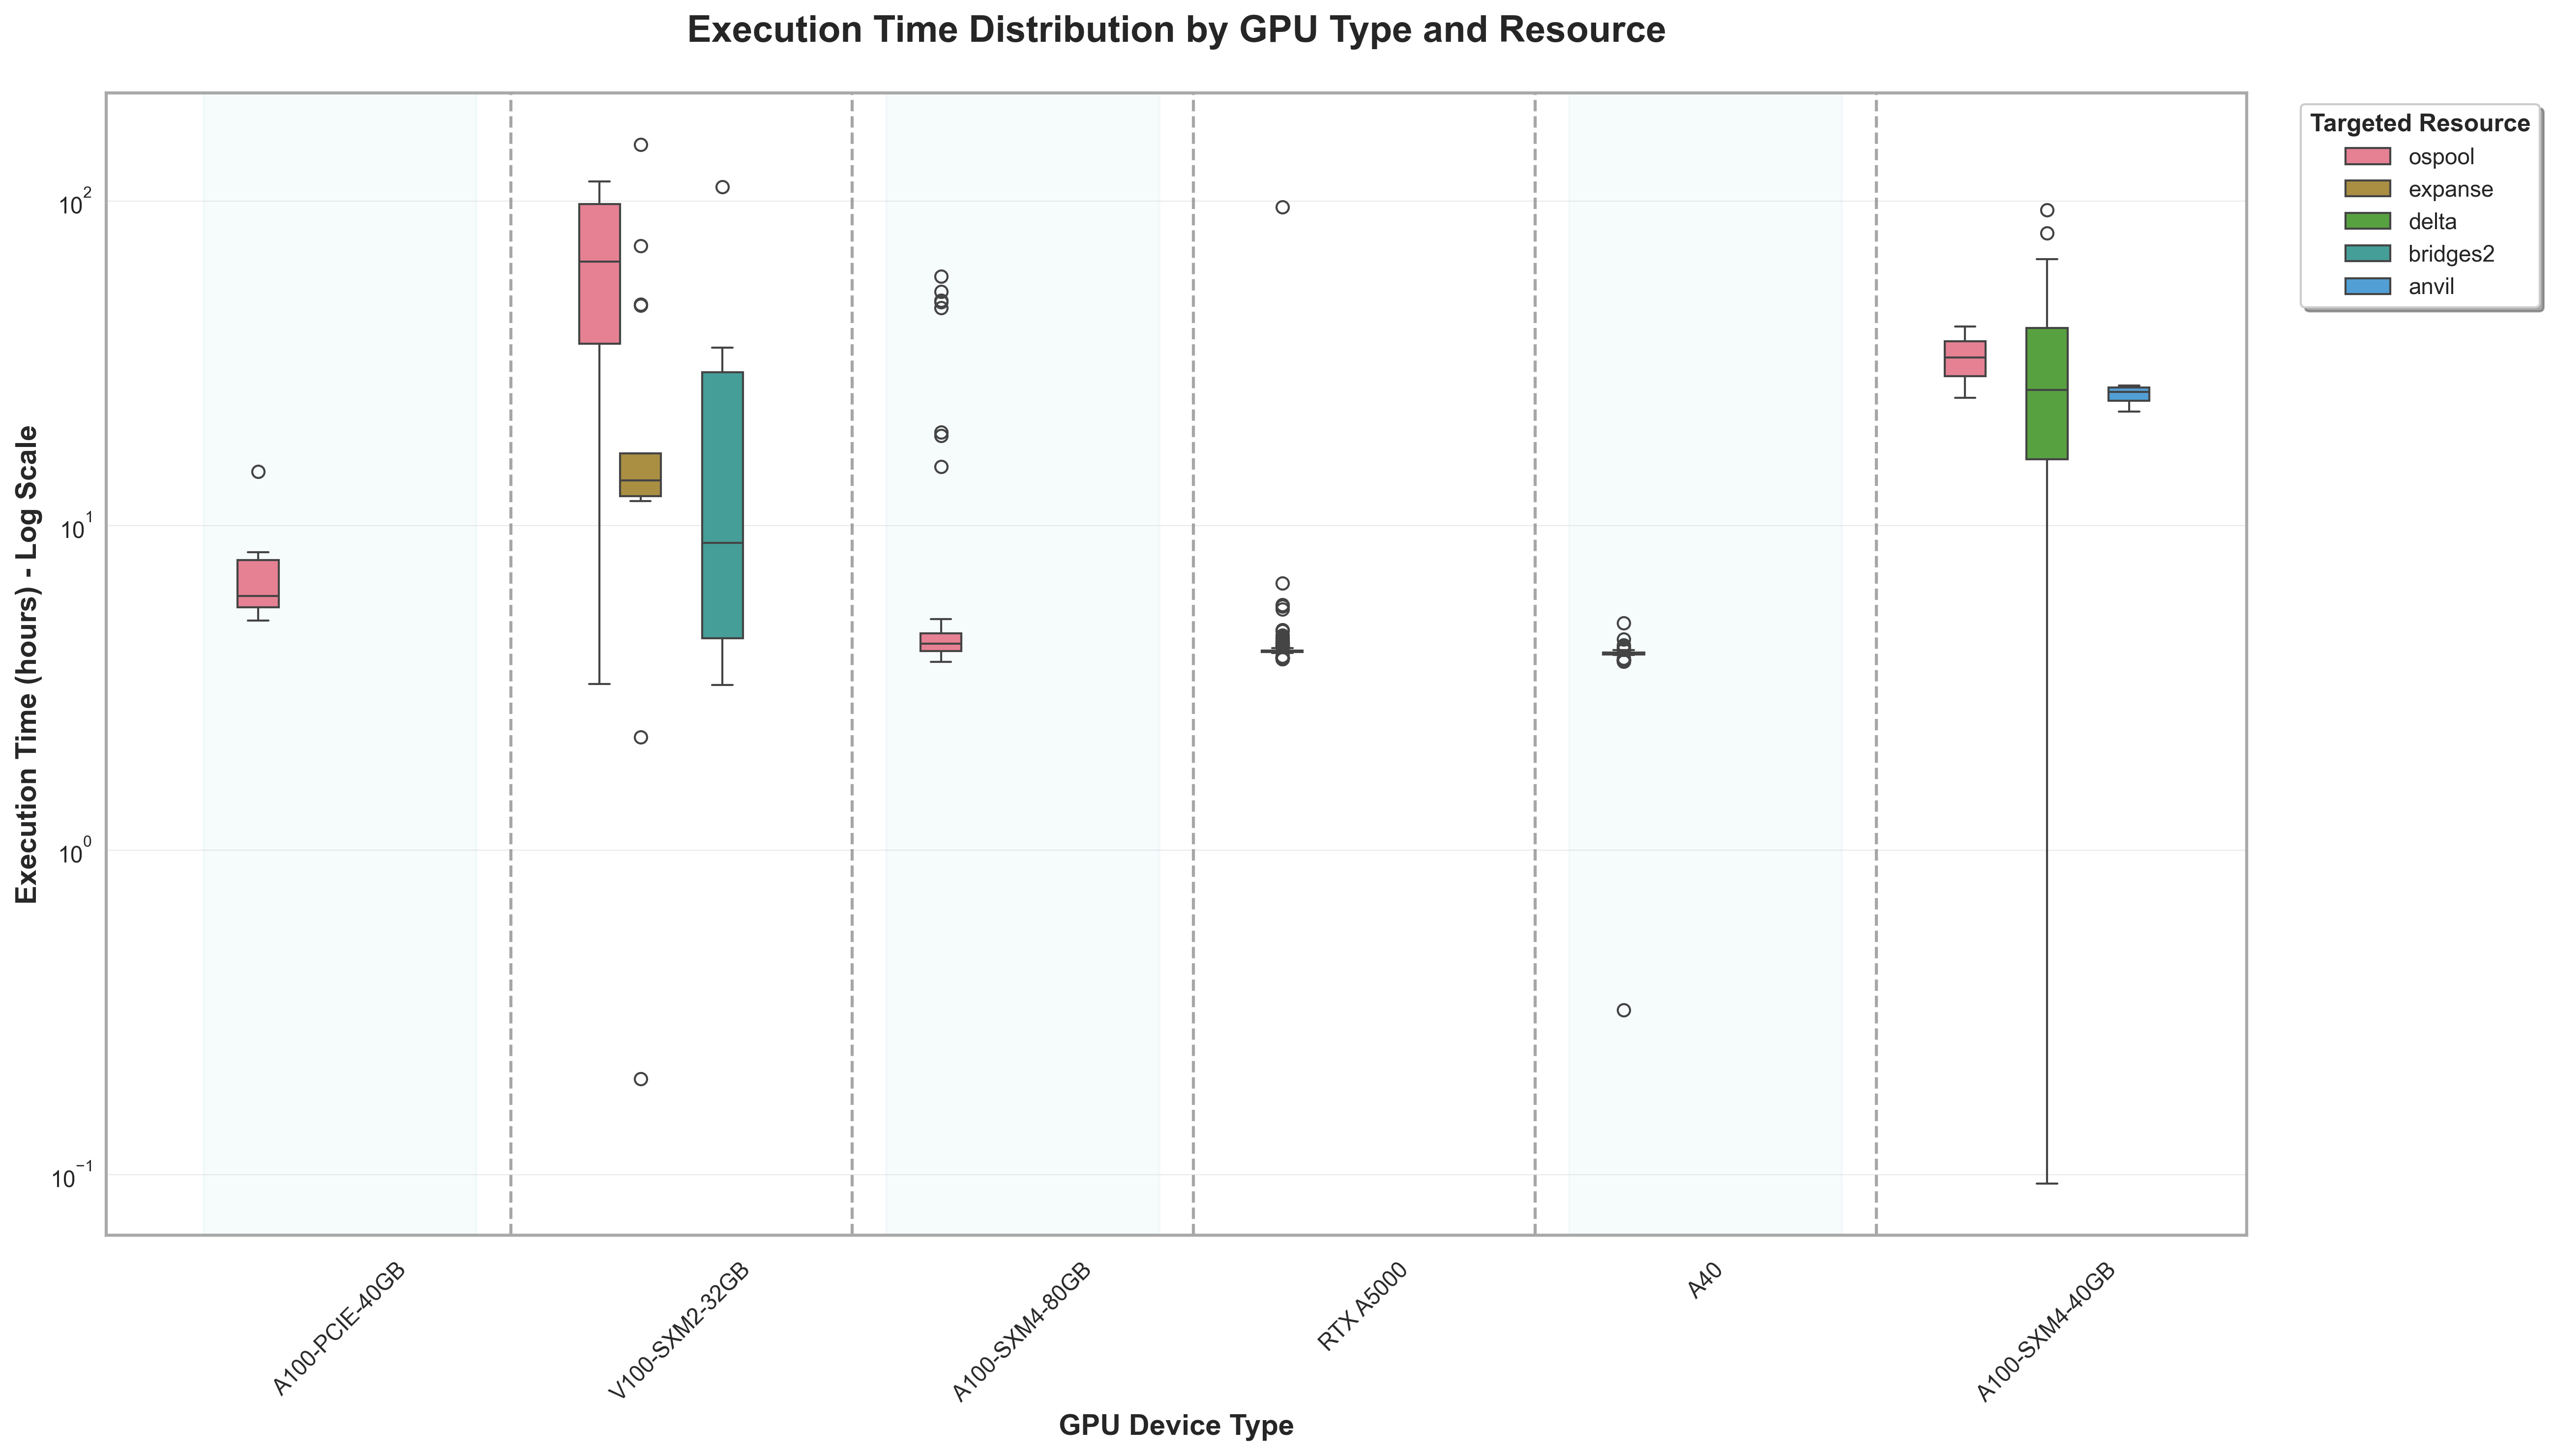
\includegraphics[width=0.8\textwidth]{gpu_runtime_by_resource_boxplot.png}
\label{fig:gpu_runtime}
\caption{Distribution of training time by GPU type and targeted resource.}
\end{figure}







\todo{}
% Add some figures:
% Epochs per resource
% Time per resource
% GPU breakdowns

\subsubsection{Evaluation}\label{results_evaluation}
Once training was completed, the model variants were evaluated using validation data. \todo{More info here.} The results are shown in Figure \ref{fig:key_metrics}.

\begin{figure}[h]
\centering
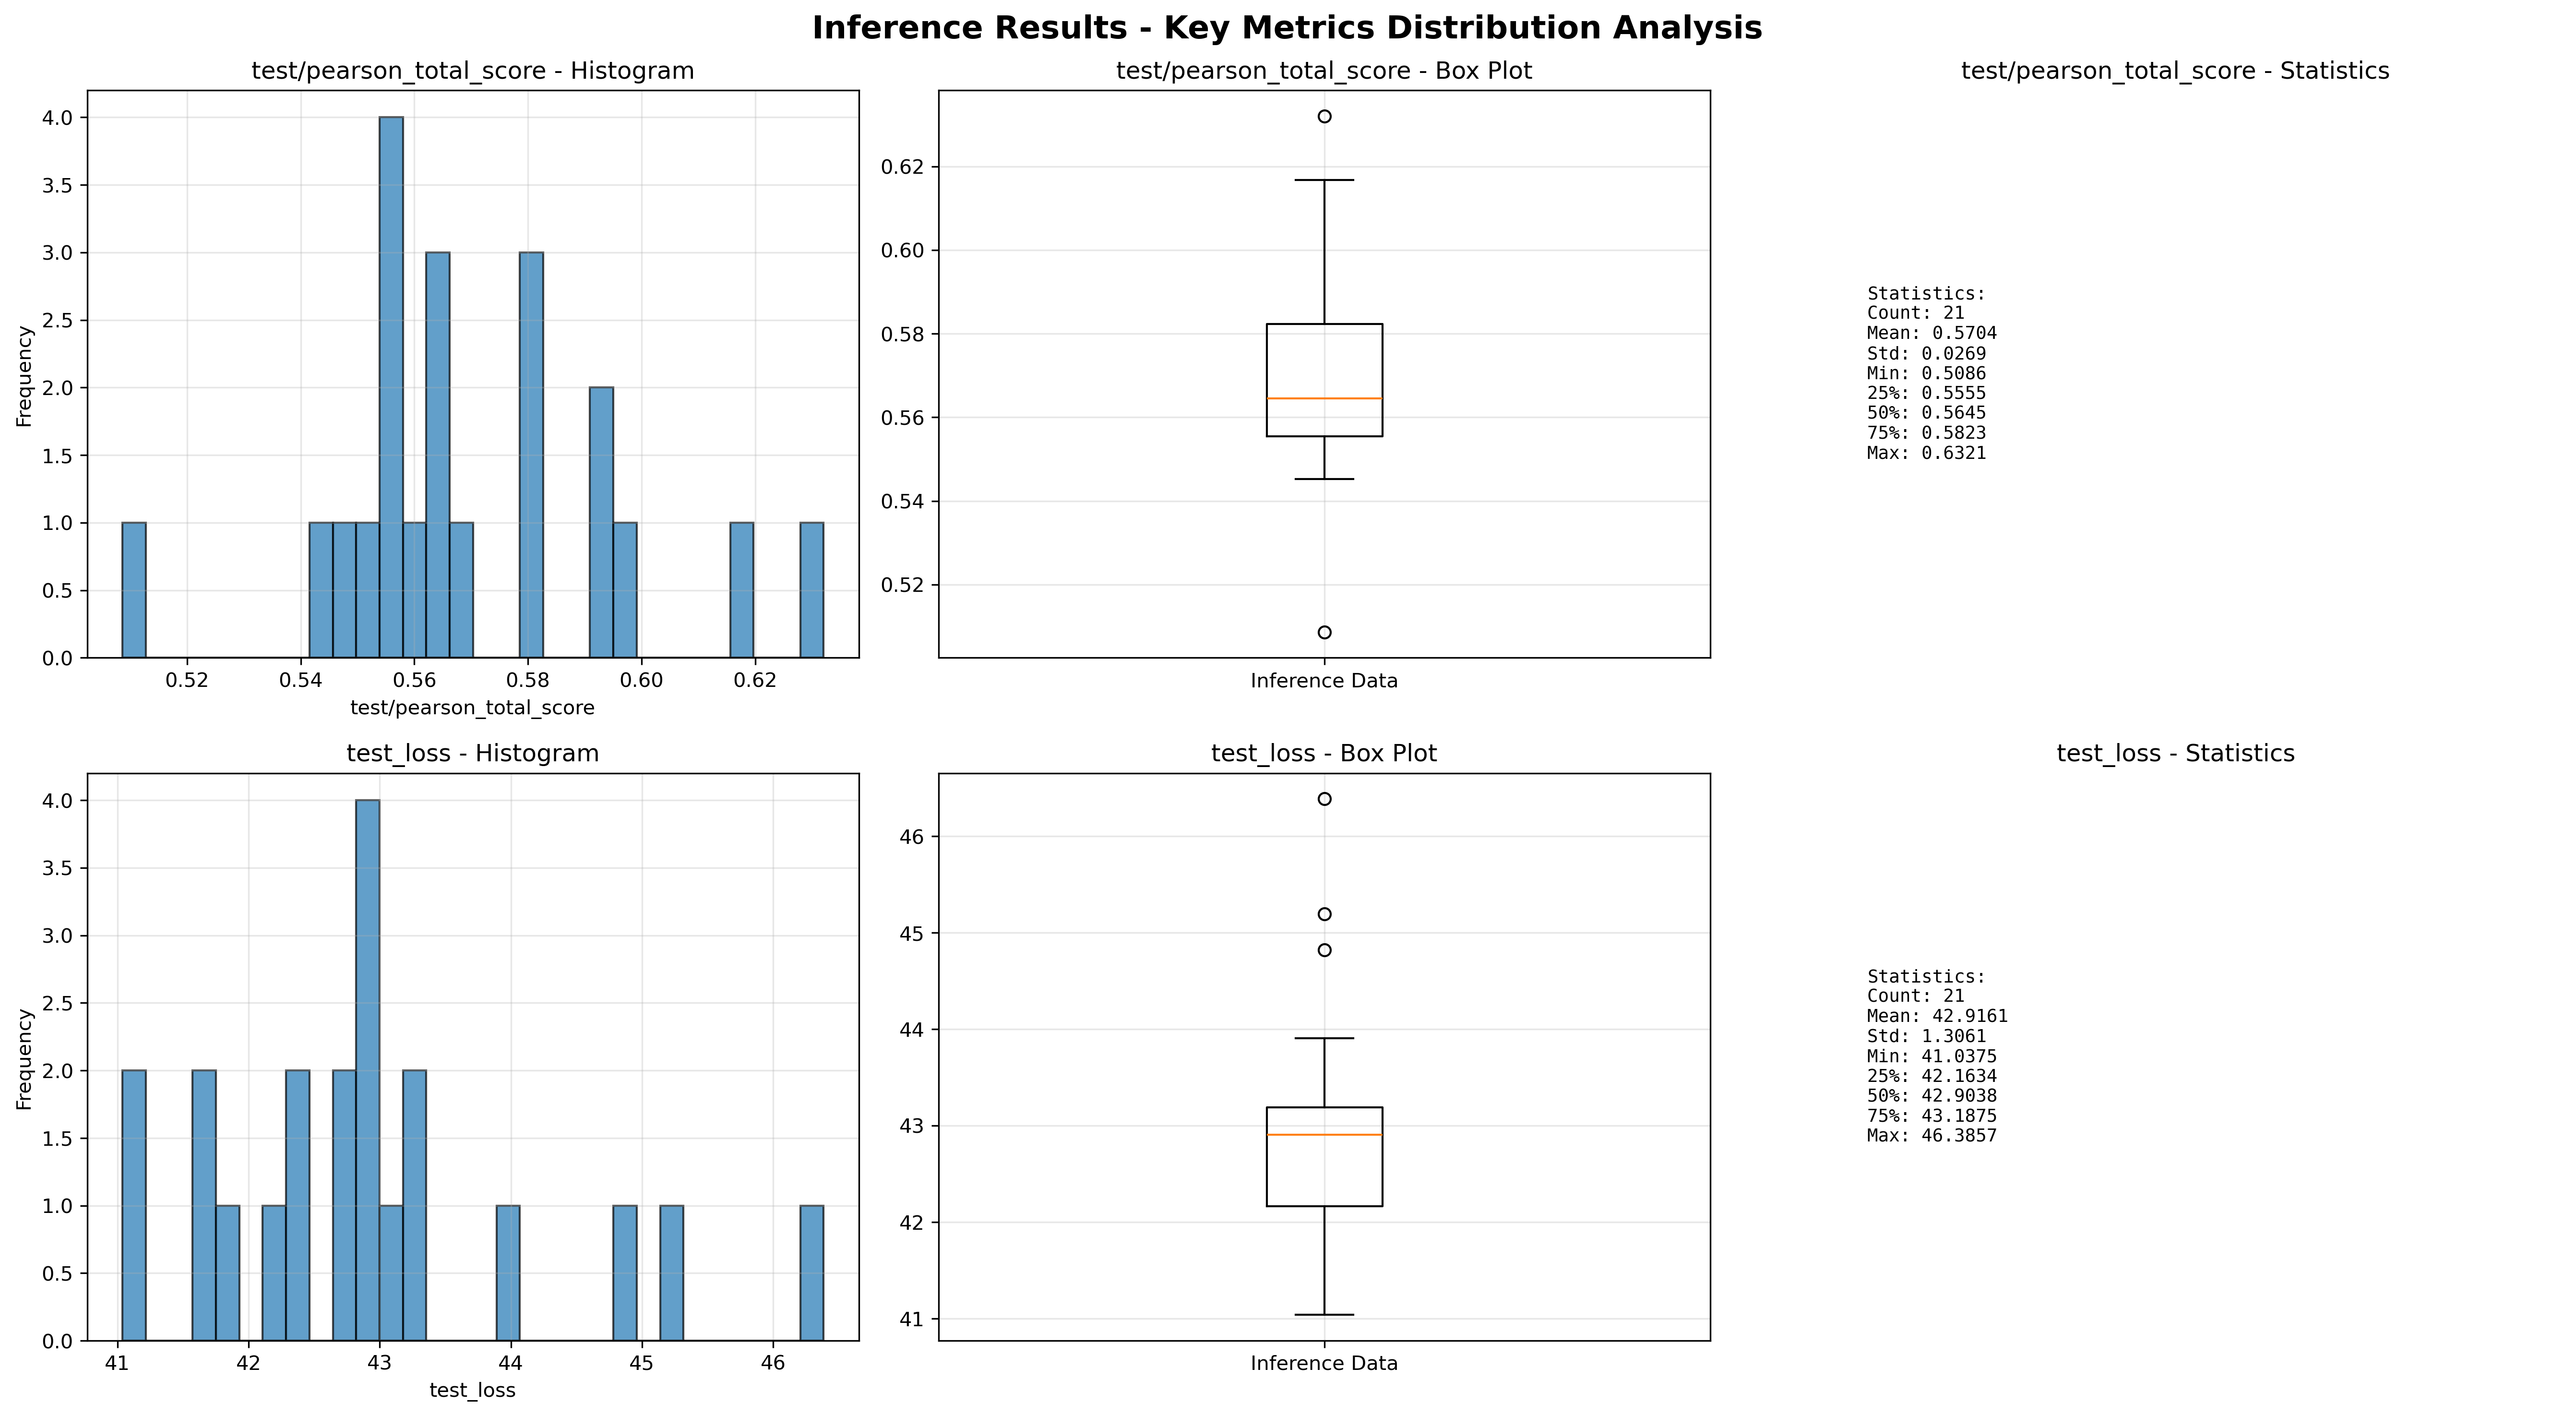
\includegraphics[width=0.8\textwidth]{plots/key_metrics_combined.png}
\label{fig:key_metrics}
\caption{Evaluation results of the 21 model variants. Pictured is comparisons of the Pearson total (top) and test loss (bottom) scores.}
\end{figure}

\begin{figure}[h]
\centering
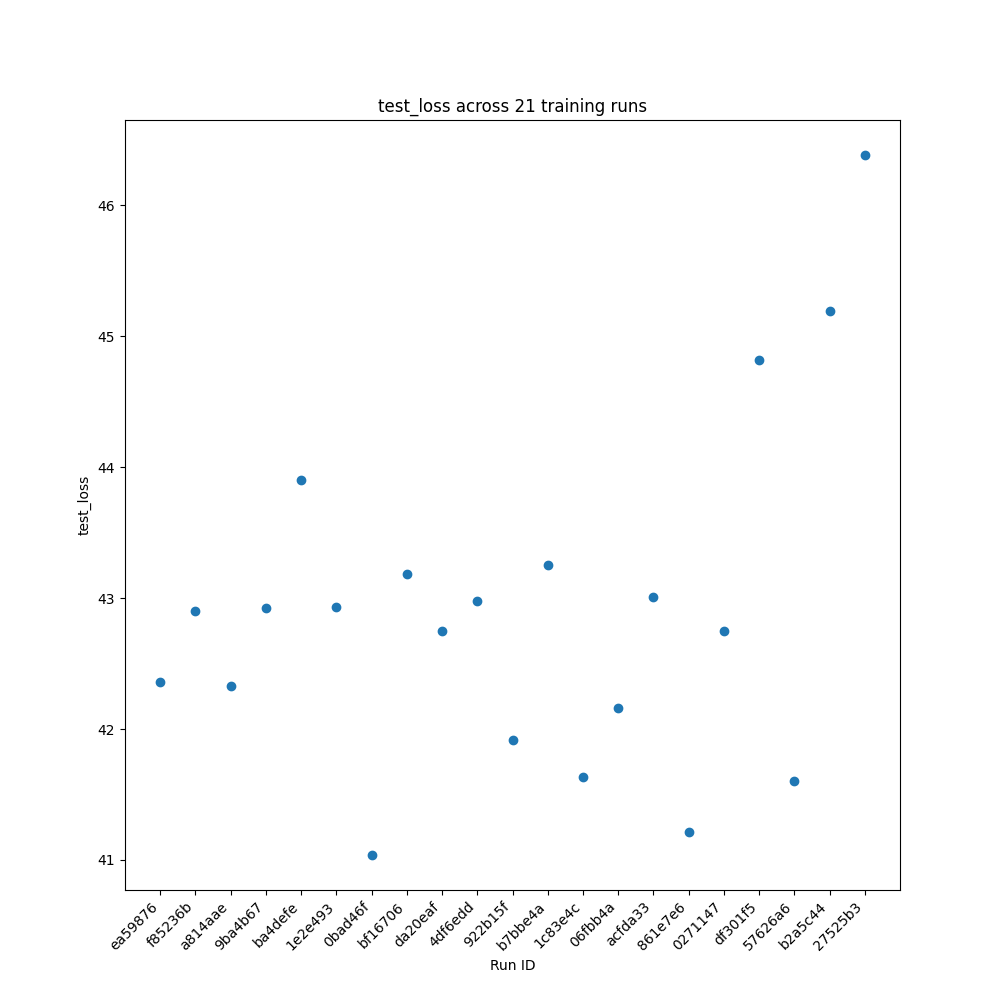
\includegraphics[width=0.48\textwidth]{plots/scatterplot_test_loss.png}
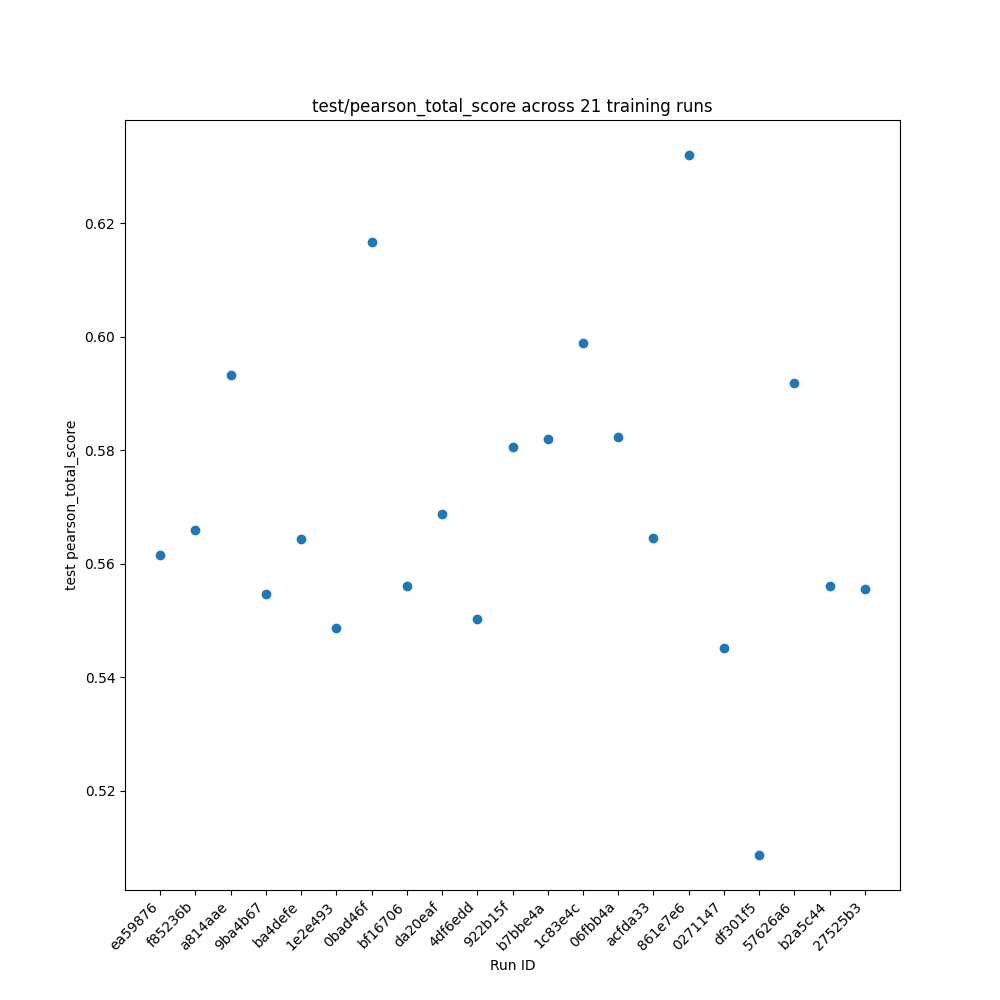
\includegraphics[width=0.48\textwidth]{plots/scatterplot_test pearson_total_score.png}
\label{fig:key_metrics}
\caption{Test loss (left) and Pearson total score (right) for the 21 model variants (by unique identifier of model)}
\end{figure}

\todo{what impact has it made?}

\subsection{Conclusions}\label{conclusions}
\subsubsection{General considerations}
For a model of this size (2.5M parameters), the OSPool is an excellent source of
GPUs available for training. The limited system and video memory needs are
easily available within capacity donated to the OSPool, allowing for efficient
training and optimization. It was not atypical for up to a dozen epochs to be training simultaneously,
allowing for substantial overall throughput in the training process.

The NAIRR sites also contributed significant computing resources, but they were
not as heavily utilized as the OSPool due to the challenges in creating uniform
and consistent pressure for jobs to consume existing annexes. The shape of the
overall training process (where epochs moved across sites, often with long gaps
between re-visiting a NAIRR resource, an annex retired before being re-utilized
by additional jobs. This created a substantial bottleneck, as re-establishing
the annex required manual intervention (due to the need for two-factor
authentication).

The overall behavior of the training process was difficult to characterize, and
similar hardware across different sites resulted in significantly different
training times. Attempts to troubleshoot this behavior was largely unsuccessful
and was attributed to an imbalance between the CPU and GPU quanities requested
within each job (e.g. creating a job with multiple GPUs at a NAIRR site, but
insufficient CPU resources to feed data to the GPUs). Troubleshooting attempts
included manually logging into the NAIRR sites and submitting the work directly
to the SLURM clusters there (to eliminate potential HTCondor/Annex impact),
moving data from the job directory to dedicated solid state space before
training, and modifying batch sizes. Little impact was observed from these
changes.

An innate challenge to adaptation of existing training workflows into a new
environment is the unfamilarity and ``black box'' nature of the software, which
substantially complicates the ability to understand and investigate significant
behavioral differences in heterogeneous environments.

\subsubsection{DAG generation and pattern repetition}
A patter that is often repeated in machine learning training is the need to run
multiple training jobs with differing configurations. Ensembles of models,
including experiments such as this project, and hyperparameter tuning are common
uses cases that fall into this category of high numbers of ``shish-kebab''
shaped workflows. Between training runs, variables or parameters may be altered
in order to optimize the model's performance, test model architecture behavior,
or to generate a group of similar models for comparison.

While creating the DAG generation script, we considered shortcomings and areas
for improvement in the HTCondor software, especially in its Directed Acyclic
Graph manager (DAGMan). While programtically creating a DAG in this fashion
is not a challenging scripting task, it is largely left to individual researchers
to re-implement similar patterns in order to capture desired behavior.

DAGMan provides handles that are useful for this kind of work, such as being
able to assign VARS at the NODE level, which allows for easily changing parameters
between training runs. However, this must be done at the level of individual nodes, resulting
in a verbose overall DAG definition that cannot easily be updated if needed. DAGMan also
provides a way to define a subdag, which allows for repeated shapes within
the overall workflow, but again lacks the flexibility in changing VARS within repetitions
of the shape.

Being able to define subdag- or region-define variables would simplify the
overall structure of the DAG file, enabling more concise and maintainable DAG
definitions. Finally, hyperparameter sweeps, a very common operation in ML
training, involves systematic explorations of a phase space. DAGMan lacks the
ability to easily program "sweeps" of values, such as letting a VAR run from
0.01 to 0.1 in steps of 0.01. Should that feature be added, concise DAG definitions
for complex ML training workflows could easily be created and utilized, instead of
multiple ala carte solutions being created by research groups.

A concise description of a DAG with SUBDAG repetition and sweeps could look something like:

\begin{verbatim}
train.subdag
PARENT {run}-train_epoch0 CHILD {run}-train_epoch1
PARENT {run}-train_epoch0 CHILD {run}-eval_epoch1
PARENT {run}-train_epoch1 CHILD {run}-train_epoch2
PARENT {run}-train_epoch1 CHILD {run}-eval_epoch2
VARS {run}-train_epoch0 epoch=1 a={a} b={b}
VARS {run}-train_epoch1 epoch=2 a={a} b={b}
VARS {run}-train_epoch2 epoch=3 a={a} b={b}
\end{verbatim}


\begin{verbatim}
workflow.dag
GEN SUBDAG train_flow train.subdag a, b from
  0.01 to 0.1 by 0.01
  0.5 to 5 by 0.5
PARENT init CHILD train_flow
\end{verbatim}

This defined a ``shish-kebab'' training subdag, with parent-child relationships
defined between epochs (with sidecar evaluation nodes). a and b represent
parameters that change between training runs but are consistent within each run.
A GEN command will generate the overall workflow, letting the values of a and b
run over their respective ranges. Finally, an initializing node (init, included
but not defined) defines any initialization that needs to happen for the
workflow as a whole and serves as a PARENT node to the training runs.


\subsubsection{Annex readiness for distributed machine learning training}
While HTCondor Annex provides a unified interface to HPC systems that provide
NAIRR allocations, the particular challenge of intentionally shifting training
between sites is somewhat at odds with the intended Annex goal of ``bursting''
into a single HPC site to provide additional short-term computing resources.
Instead, there was non-constant pressure of jobs targeting each site, resulting
in constant annex retirement and the need for re-identification (often with
two-factor authentication) at each site to re-establish the annex and continue
training. This prevented full automation of the training process, as manual
intervention was often required. Constant pressure (for example, from targeting
only one NAIRR resource) could certainly solve this problem, with HTCondor
providing the organization and management aspects of the training run.
\subsubsection{Future work}
\todo{second experiment, updated model config, ...}


\subsection{Appendix}\label{section-1}
\subsubsection{Woes and Findings}
\todo{Training speed}


\end{document}
